\thispagestyle{fancy}
\vspace*{40 pt}
\subsection{Tela comando slotter}
 Esta tela é acessada pelo botão "\textgreater" no menu superior esquerdo da tela de comando da ultima impressora, pelo botão "\textless{}" no menu superior esquerdo da tela comando perfuradora, pelo botão "SLT" em qualquer tela de comando e pelo botão comando da tela ajustes slotter.
 \vspace*{\fill}
 \begin{figure}[h]
  \centering
  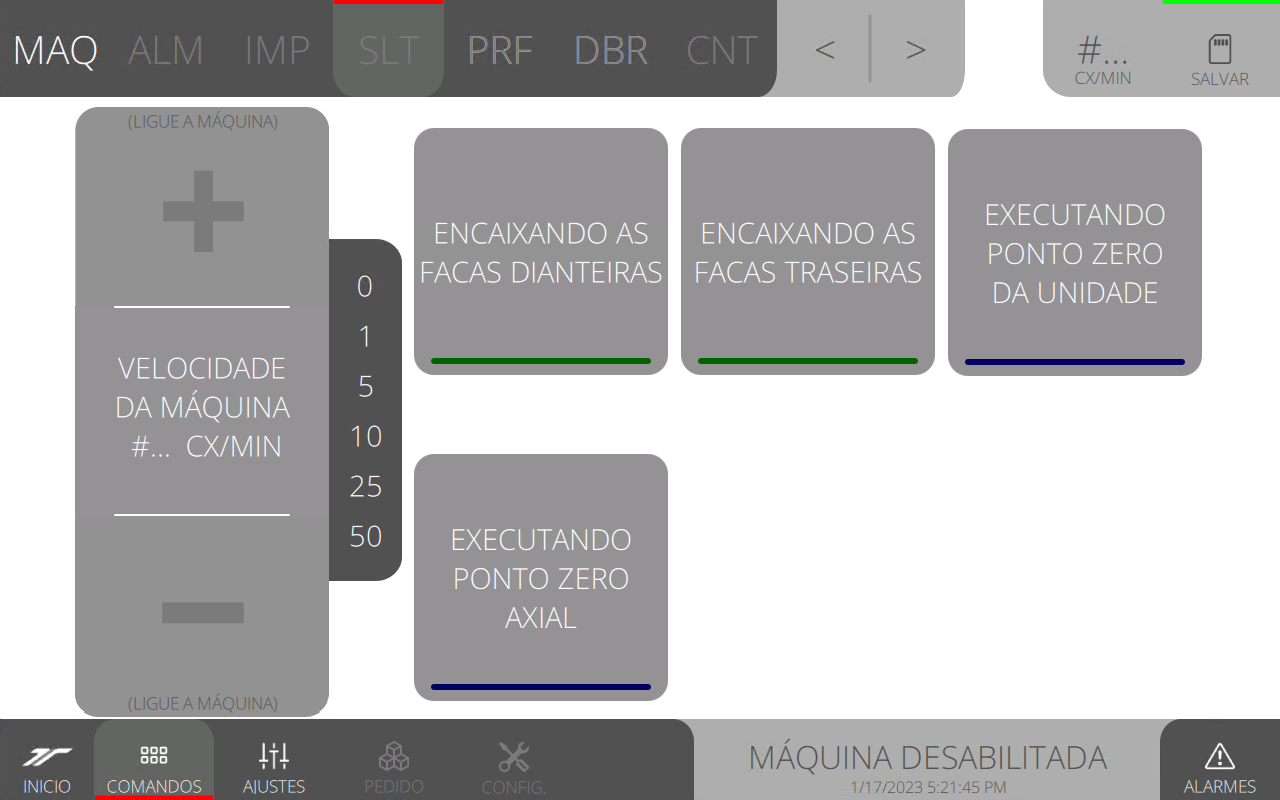
\includegraphics[width=576px,height=360px]{src/imagesFlexo/05-slotter/commands/e-Tela-Principal.png}
\end{figure}
\vspace*{\fill}

\newpage
\thispagestyle{fancy}
\vspace*{40 pt}
\subsubsection{\small{Encaixe das facas traseiras}}
\vspace*{\fill}
\begin{figure}[h]
  \centering
  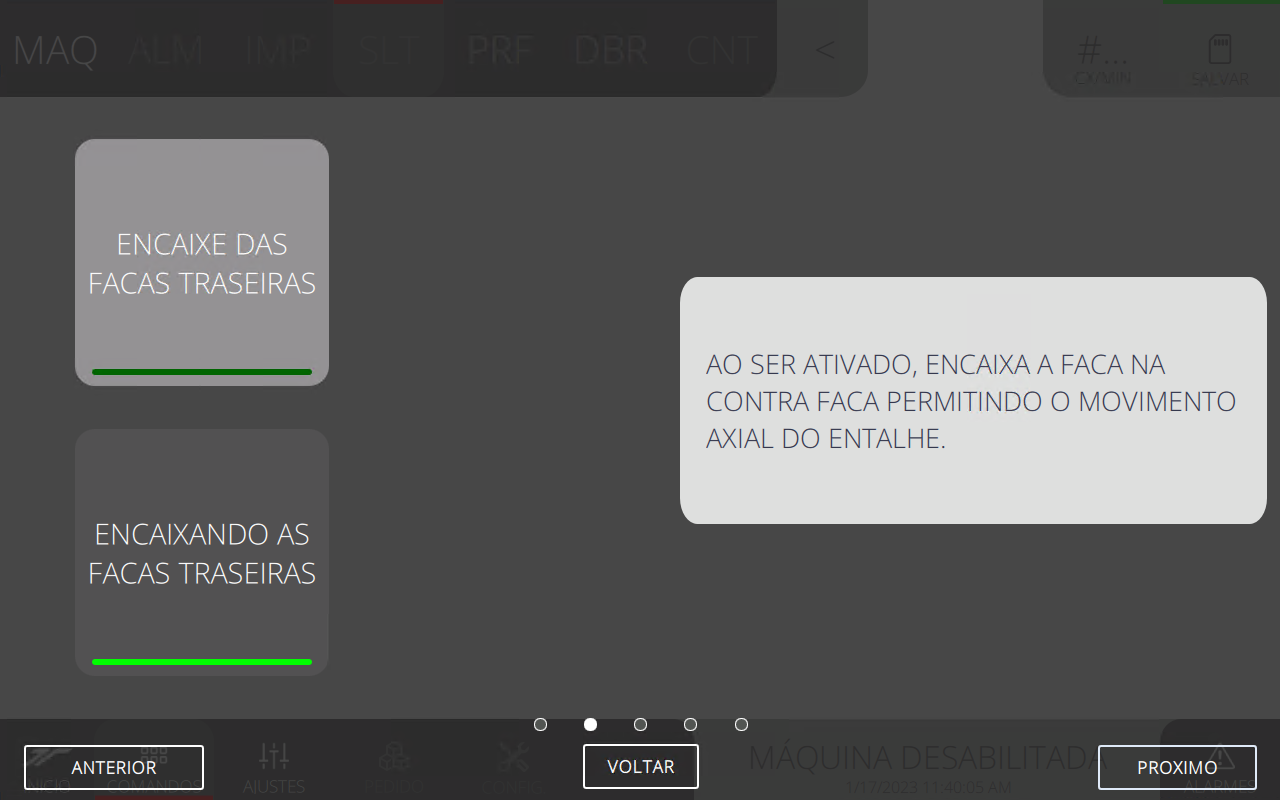
\includegraphics[width=576px,height=360px]{src/imagesFlexo/05-slotter/commands/e-2.png}
\end{figure}
\vspace*{\fill}

\newpage
\thispagestyle{fancy}
\vspace*{40 pt}
\subsubsection{\small{Executa ponto zero da unidade}}
\vspace*{\fill}
\begin{figure}[h]
  \centering
  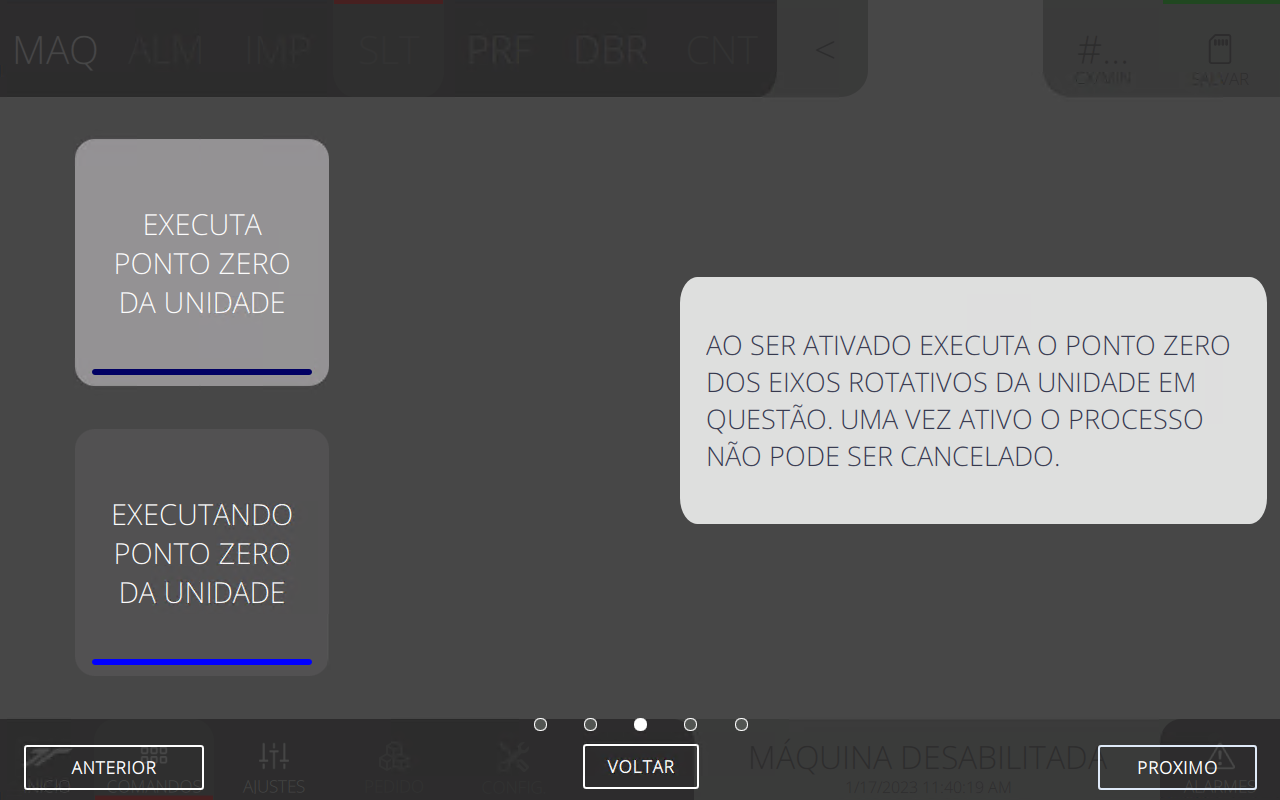
\includegraphics[width=576px,height=360px]{src/imagesFlexo/05-slotter/commands/e-3.png}
\end{figure}
\vspace*{\fill}


\newpage
\thispagestyle{fancy}
\vspace*{40 pt}
\subsubsection{\small{Executa ponto zero axial}}
\vspace*{\fill}
\begin{figure}[h]
  \centering
  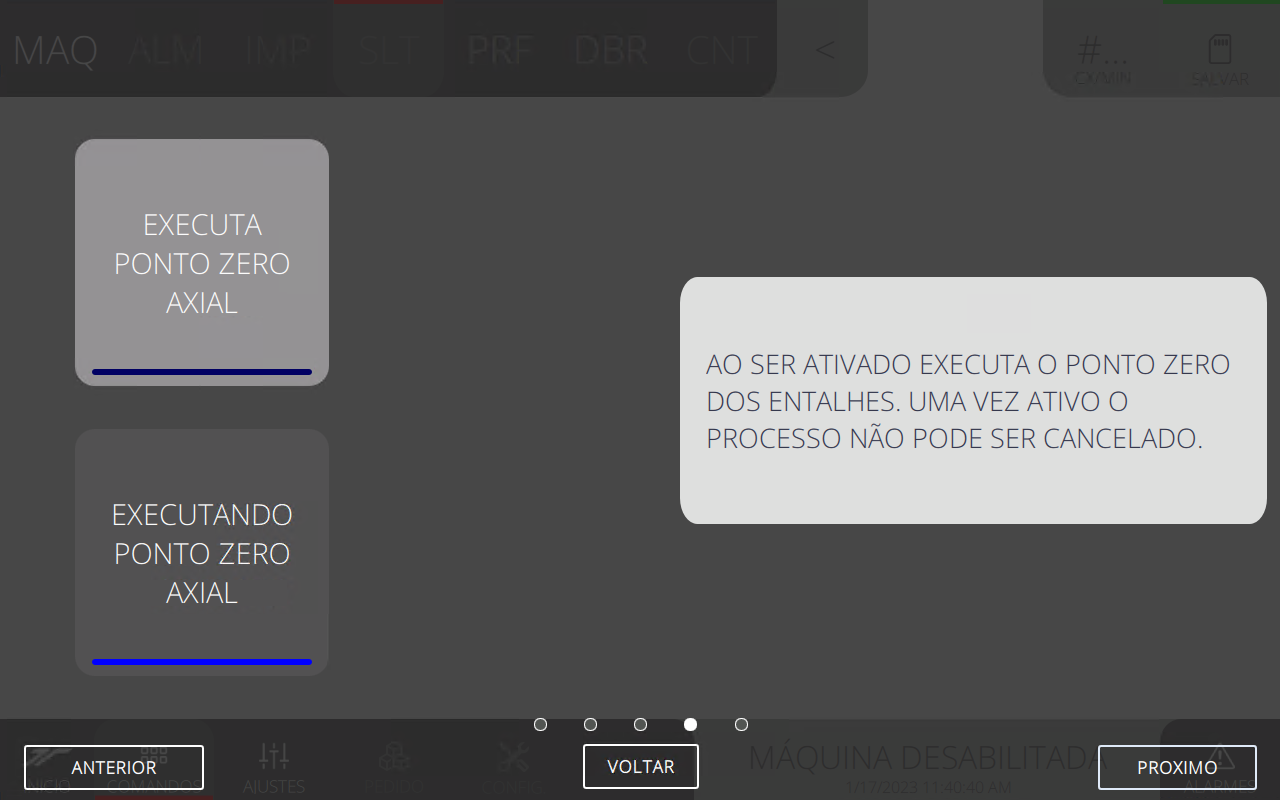
\includegraphics[width=576px,height=360px]{src/imagesFlexo/05-slotter/commands/e-4.png}
\end{figure}
\vspace*{\fill}

\newpage
\thispagestyle{fancy}
\vspace*{40 pt}
\subsubsection{\small{Encaixe das facas dianteiras}}
\vspace*{\fill}
\begin{figure}[h]
  \centering
  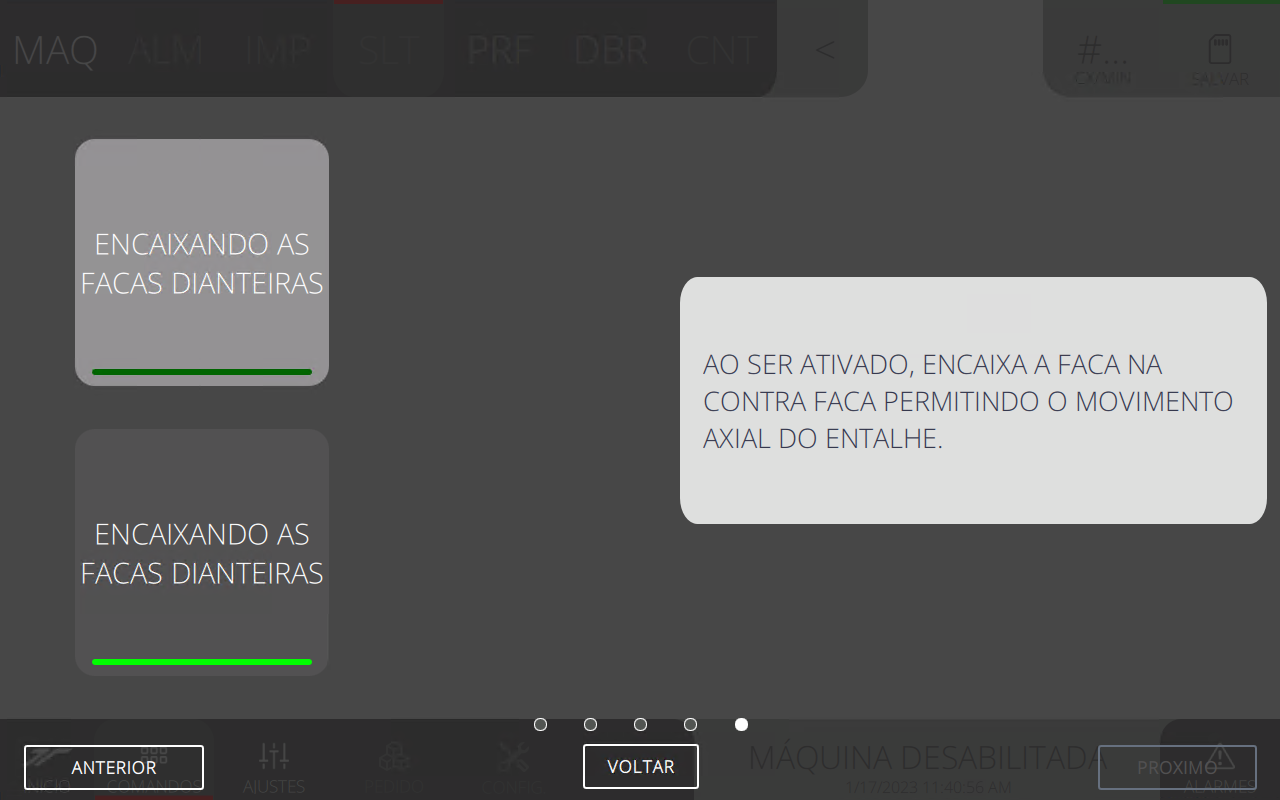
\includegraphics[width=576px,height=360px]{src/imagesFlexo/05-slotter/commands/e-5.png}
\end{figure}
\vspace*{\fill}

